\section{Ruler: Rewrite Synthesis using Equality Saturation}

\newcommand{\rationals}{{rationals}\xspace}
\newcommand{\bfour}{{bitvector-4}\xspace}
\newcommand{\bthreetwo}{{bitvector-32}\xspace}
\newcommand{\booleans}{{booleans}\xspace}
\newcommand{\ints}{ℤ}
\newcommand{\reals}{ℝ}
\newcommand{\ruler}{Ruler\xspace}
\newcommand{\Ruler}{Ruler\xspace}
\newcommand{\cvec}{cvec\xspace}
\newcommand{\cvecs}{cvecs\xspace}


\lstdefinestyle{ruler}{
  basicstyle=\footnotesize\sffamily,
}
\lstset{
  style=ruler,
  commentstyle=\sffamily\itshape,
  columns=fullflexible,
  showstringspaces=false,
  % literate={-}{--}{1},
  % numbers=left,
  xleftmargin=0em,
  mathescape,
  language=Python,
  morekeywords={loop},
}

\begin{figure}
  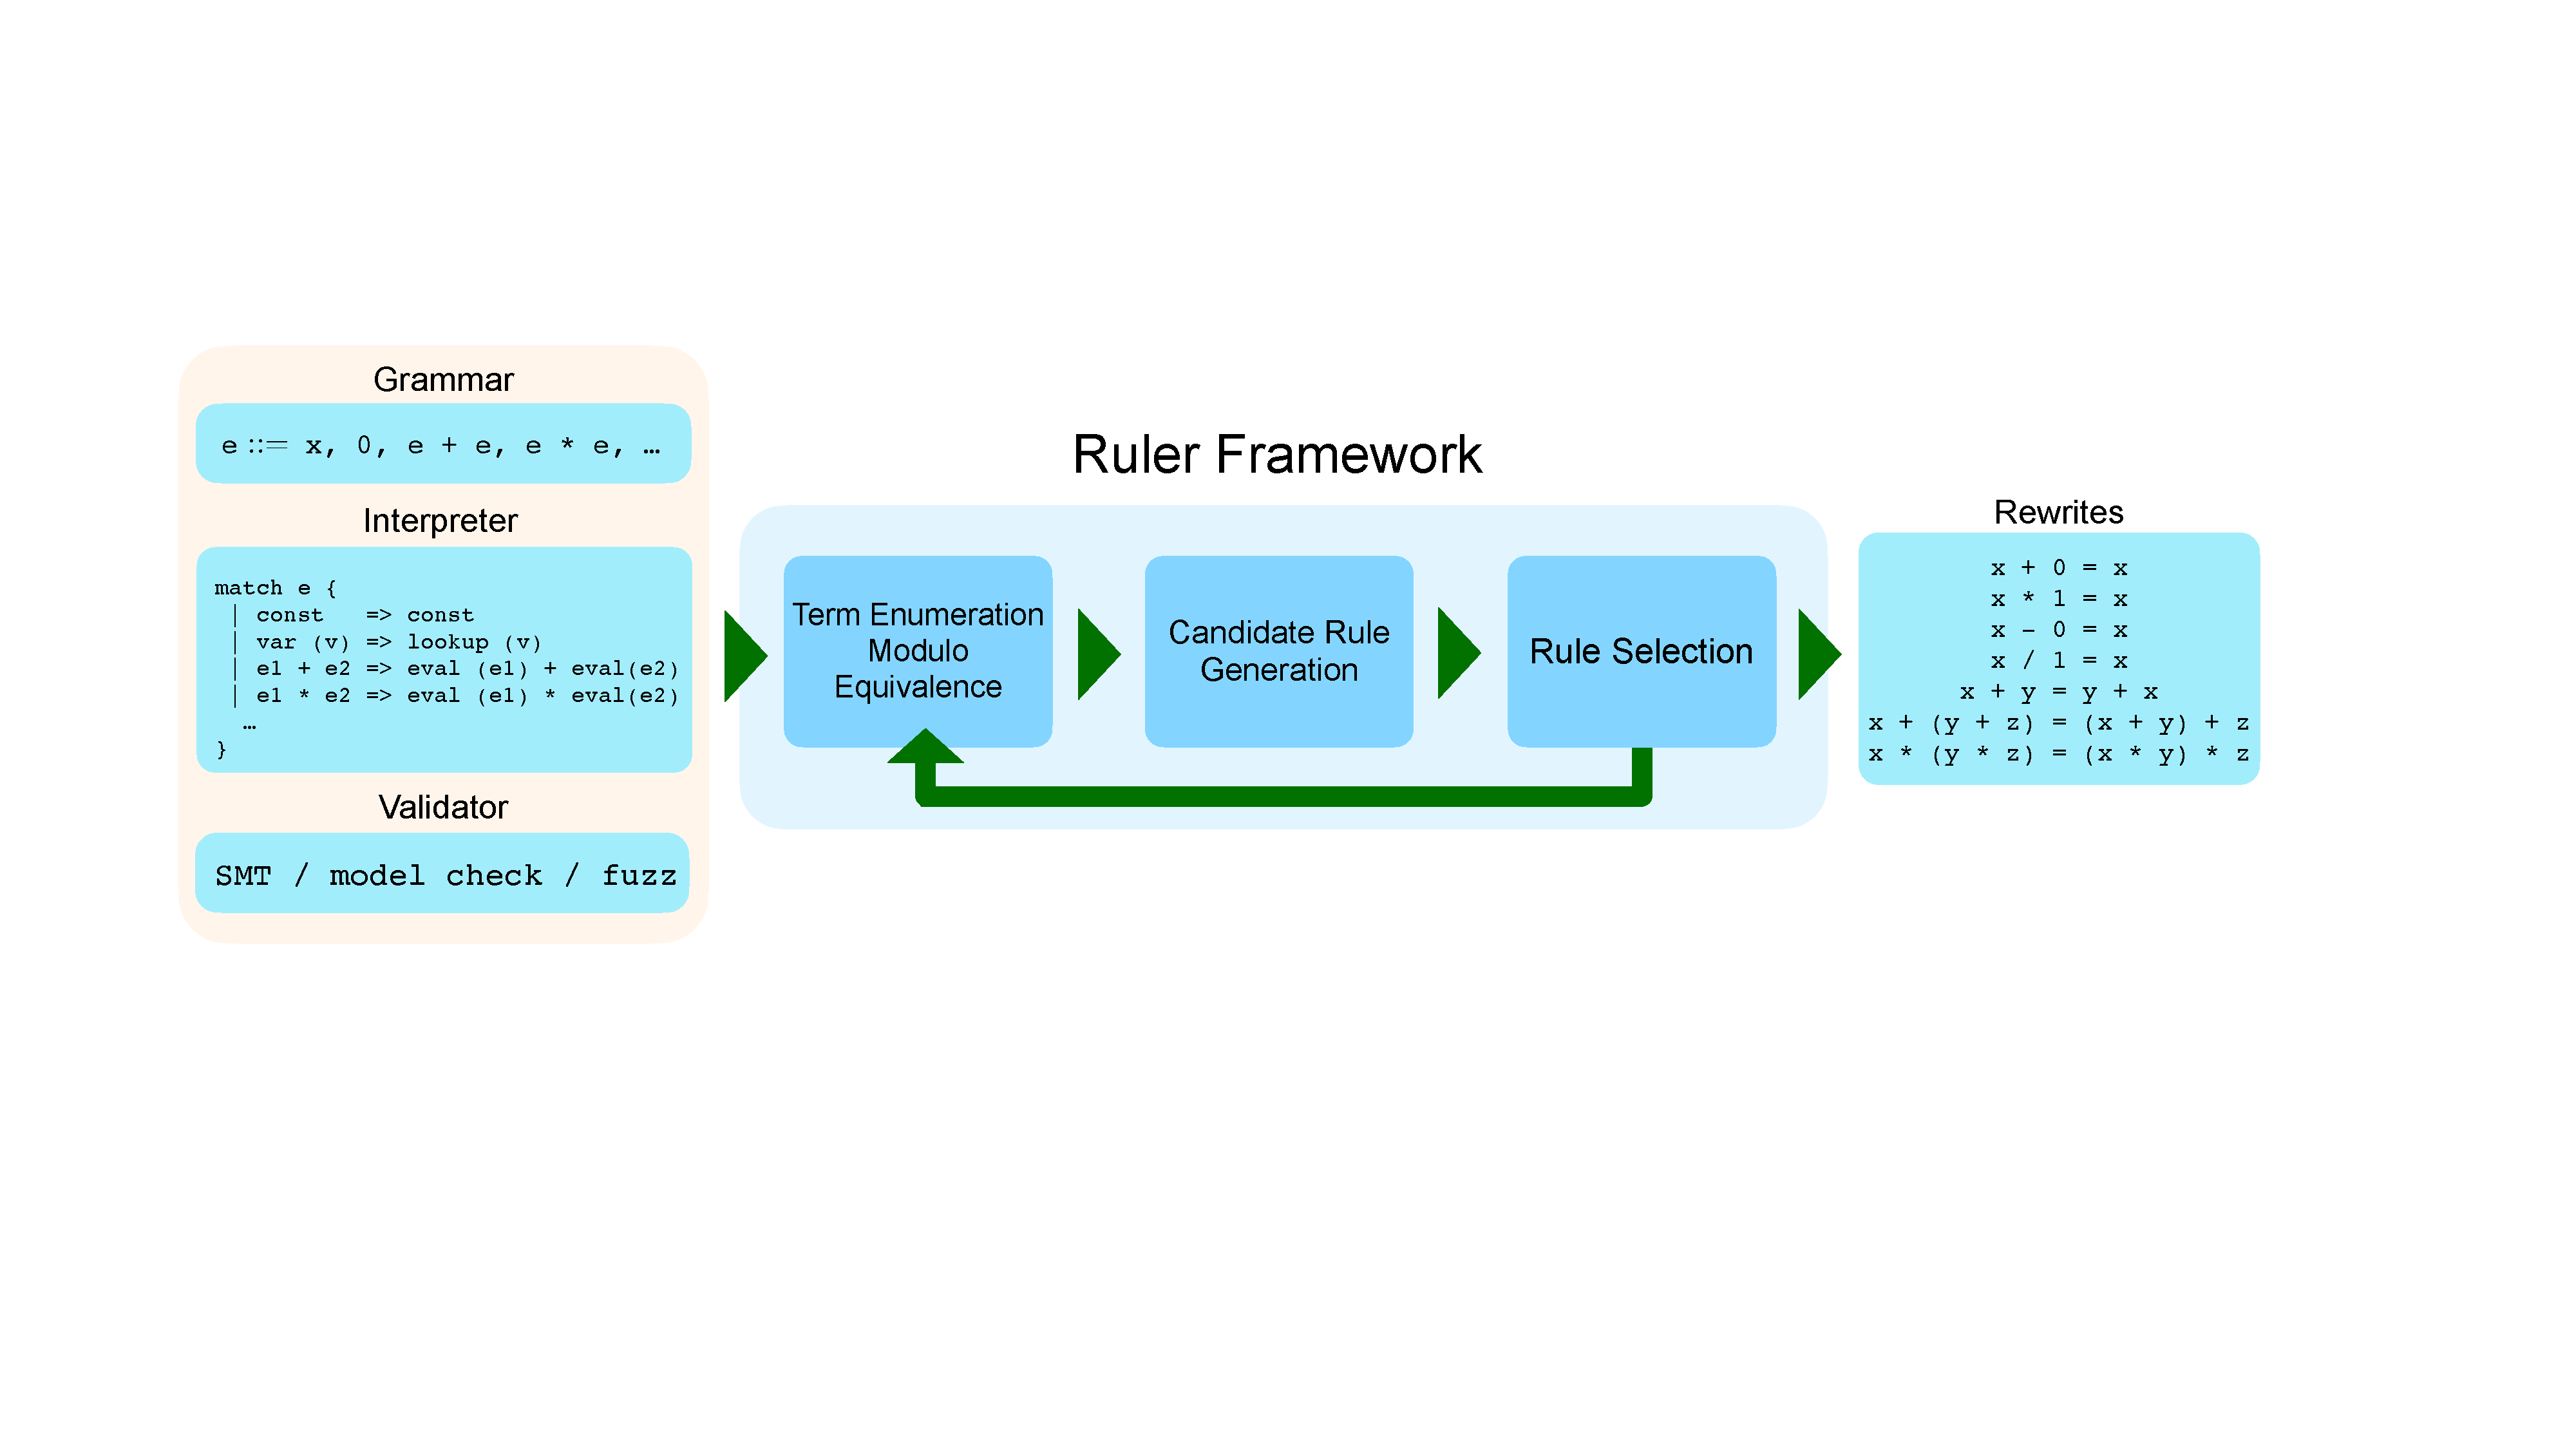
\includegraphics[width=\textwidth]{ruler-workflow.pdf}
  \caption{
    \textit{\ruler Workflow}.
    Given a grammar and interpreter for a target domain,
    \ruler uses e-graphs and equality saturation
    to efficiently enumerate potential rewrite rules and
    iteratively select a small set of general, orthogonal rules.
    \ruler supports various validation strategies to
    ensure soundness and speed up synthesis, including
    constraint solving (e.g., SMT), model checking, and fuzzing.
  }\label{fig:ruler}
\end{figure}

Many compilers, program synthesizers, and theorem provers
  rely on rewrite systems~\cite{
    haskell, arvind-hw-synth-rw, simplify}.
For example, rewriting is essential for
  improving program analyses and code generation~\cite{
    isel-survey, mlir, halide, tvm}
  and for automating verification~\cite{
    cvc4, z3, isabelle, coq}.
Without rule-based simplification,
  Halide-generated code can
  suffer $26\times$ slowdown~\cite{julie-halide}
  and
  the Herbie floating-point synthesizer~\cite{herbie}
  can return $10\times$ larger programs.

Where do the rewrite rules come from?
Several noteworthy projects have developed
  tool-specific techniques for checking or inferring rules~\cite{
    bansal, alive-infer, denali, swapper},
  but %, despite their importance,
  implementing a rewrite system
  still generally requires domain experts to
  first manually develop rulesets by trial and error.
Such slow, ad hoc, and error-prone approaches
  hinder design space exploration for new domains
  and discourage updating existing systems.


To address these challenges,
  we propose a simple, domain-general approach
  that uses \eqsat~\cite{eqsat, egg} as
  a rewrite system \textit{on the domain of rewrite rules themselves}
  to quickly synthesize effective rulesets.

In the past, tool-specific techniques
  to iteratively infer rewrite rules
  have implicitly adopted a common three-step approach,
  each constructing or maintaining a set:
\begin{enumerate}
    \item Enumerate terms from the given domain to
          build the \textit{term set} $T$.
    \item Select candidate rules from $T \times T$
          to build the \textit{candidate set} $C$.
    \item Filter $C$ to select a sound set of
          useful rules to build the \textit{rule set} $R$.
\end{enumerate}
We identify and abstract this workflow
  to provide generic rule inference for user-specified domains.

Our key insight is that \emph{what
  makes \eqsat successful in rewrite rule application
  is also useful for rule inference}.
\Eqsat can simultaneously prove many pairs of terms equivalent
 with respect to a given ruleset.
\ruler uses \eqsat to shrink
  the set $T$ of enumerated terms
  (lowering candidate \textit{generation} cost)
    by merging terms equivalent under $R$,
    and to shrink the set $C$ of candidate rules
  (lowering candidate \textit{selection} cost)
    by removing rules derivable by $R$.
Thus, \ruler uses the set $R$ of rewrite rules
  to rewrite the next batch of candidate rewrite rules
  \textit{even as $R$ is being synthesized}.


We prototyped these insights in
  a tool dubbed \ruler (\autoref{fig:ruler}).
Compared to a state-of-the-art
 rule synthesizer \cite{sat19} built
 into the CVC4 theorem prover~\cite{cvc4},
  Ruler synthesizes smaller rulesets in less time
  without reducing the set of derivable equivalences.
We demonstrate how \ruler
  can generate expert-quality rulesets
  by using it to replace all of
  Herbie's rules for rational numbers,
  uncovering missing rules that
  resolved a known bug in Herbie.

This case study's contributions include:
\begin{itemize}
  \item A novel rule synthesis algorithm
    that uses \egraphs~\cite{nelson} to
    compactly encode large sets of terms and
    \eqsat to efficiently filter and minimize rulesets
    (\autoref{sec:ruler-core}).

  \item A generic implementation of
    this algorithm within the
    \ruler
    rewrite rule inference framework
    that synthesizes rules for user-specified domains
    given a grammar and its interpreter.

  \item A comparison against a recent CVC4-based rule synthesizer
    that shows \ruler synthesizes $5.8\times$ smaller
    rulesets $25\times$ faster without compromising
    the deriving power of the rulesets.

  \item A case study demonstrating that,
    in an end-to-end application of a real world tool,
    \ruler's automatically generated rulesets
    are as good as manually-crafted expert rules
    (\autoref{sec:ruler-herbie}).

\end{itemize}

We implemented \ruler in Rust
 using \egg~\cite{egg} for
 equality saturation.
\egg's flexibility allows \ruler to be relatively simple:
 its core consists of under 1,000 lines of code,
 allowing it to be simple, extensible,
 and generic over domains.
Compared to the rewrite synthesis tool
 inside the CVC4 solver~\cite{cvc4, sat19},
 \ruler is an order of magnitude smaller.
 % Since \ruler's core algorithm does not rely on SMT,
 % \ruler can learn rewrite rules over domains
 % unsupported by SMT-LIB~\cite{smtlib},
 % or for alternative semantics for those domains
 % \footnote{For example, the Halide~\cite{halide} tool uses division semantics where $x/0=0$;
 %  this is different from the SMT-LIB semantics, but it can easily be encoded using the \texttt{ite} operator.}
 % (\autoref{subsec:updates}).

\subsection{Ruler's Algorithm}
\label{sec:ruler-core}

Like other rule synthesis approaches,
 \ruler iteratively performs three steps:
\begin{enumerate}
    \item Enumerate terms into a set $T$.
    \item Search $T \times T$ for a set of candidate equalities $C$.
    \item Choose a useful, valid subset of $C$ to add to the ruleset $R$.
\end{enumerate}

\ruler's core insight is that \egraphs and \eqsat can help
 compactly represent the sets $T$, $C$, and $R$, leading
 to a faster synthesis procedure that produces smaller
 rulesets $R$ with greater proving power.

\begin{figure}
\begin{lstlisting}[
  basicstyle=\normalsize\ttfamily,
  xleftmargin=2.5em,
  numbers=left]
def ruler (iterations):
  $T$ = empty_egraph()                            $\label{ln:empty-egraph}$
  $R$ = $\{\}$
  for $i \in [0, \texttt{iterations}]\label{ln:iterations}$:
    # add new terms directly to the e-graph representing $T$
    add_terms($T$, $i$)     $\label{ln:add-expressions}$
    loop:$\label{line:inner-loop}$
      # combine e-classes in the e-graph representing $T$ that $R$ proves equivalent
      run_rewrites($T$, $R$)    $\label{ln:run-rewrites}$
      $C$ = cvec_match($T$)             $\label{ln:cvec-match}$
      if $C = \{\}$:
        break
      # choose_eqs only returns valid candidates by using 'is_valid' internally
      $R$ = $R\ \cup$ choose_eqs($R$, $C$)                 $\label{ln:choose-eqs}$
  return $R$
\end{lstlisting}
  \caption{
  \ruler's Core Algorithm.
  The \textsf{iterations} parameter
  determines the maximum
  number of connectives in the terms
  \ruler will enumerate.
  }
  \label{fig:ruler-core}
\end{figure}

\autoref{fig:ruler-core} shows \ruler's core
  synthesis algorithm,
  which is parameterized by the following:
\begin{itemize}
    \item The number of iterations to perform the search for (line \ref{ln:iterations});

    \item The language grammar, given in the form of a term enumerator
          (\lstinline{add_terms}, line \ref{ln:add-expressions}),
          which takes the number of variables or constants to enumerate over;
\item The procedure for validating candidate rules, \lstinline{is_valid}
          (called inside \lstinline{choose_eqs}, \autoref{fig:choose-eqs} line \ref{ln:is-valid}).
\end{itemize}

These parameters provide flexibility for
 supporting different domains,
 making \ruler a rule synthesis framework
 rather than a single one-size-fits-all tool.



Ruler uses an e-graph to compactly represent the set of terms $T$.
In each iteration,
  \ruler first extends the set $T$
  with additional terms from the target language.
Each term $t \in T$ is tagged with a
 \textit{characteristic vector} (cvec) that
 stores the result of evaluating $t$ given
 many different assignments of values to variables.


After enumerating terms,
  \ruler uses \eqsat
  (\lstinline{run_rewrites})
  to  merge terms in $T$
  that can be proved equivalent
  by the rewrite rules already discovered (in the set $R$);

Next, \ruler computes a set $C$ of candidate rules (\lstinline{cvec_match}).
It finds pairs $(t_1, t_2) \in T \times T$
  where $t_1$ and $t_2$
  are from distinct \eclasses
  but have matching \cvecs
  and thus are likely to be equivalent.
Thanks to \lstinline{run_rewrites},
  no candidate in $C$ should be derivable from $R$.
However, $C$ is often still large and
  contains many redundant or invalid candidate rules.

Finally, \ruler's \lstinline{choose_eqs} procedure picks a valid subset of $C$ to add to $R$,
  ideally finding the smallest extension
  which can establish all equivalences implied by $R \cup C$.
\ruler tests candidate rules for validity using a
 domain-specific \lstinline{is_valid} function.
This process is repeated until there are no
  more equivalences to learn between terms in $T$,
  at which point \ruler begins another iteration.

% \subsection{Enumeration Modulo Equivalence}
% \label{subsec:por}

% Rewrite rules encode equivalences between terms,
%   often as relatively small ``find and replace'' patterns.
% Thus, a straightforward strategy for
%   finding candidate rules is to
%   find all equivalent pairs of terms up to some maximum size.
% Unfortunately,
%   the set of terms up to a given size grows exponentially,
%   making complete enumeration impractical for many languages.
% This challenge may be mitigated by
%   biasing enumeration towards ``interesting'' terms,
%   e.g. drawn from important workloads, or by
%   avoiding bias and using sampling techniques to
%   explore larger, more diverse terms.
% \ruler can support both
%   domain-specific prioritization and random sampling
%   via the \lstinline{add_terms} function.
% While these heuristics can be very effective,
%   they often risk missing profitable candidates
%   for new classes of inputs or use cases.


% Term space explosion can also be mitigated by
%   partitioning terms into equivalence classes
%   and only considering a single, canonical
%   representative from each class.
% Similar to partial order reduction techniques in
%   model checking~\cite{peled1998ten}
%   this can make otherwise intractable enumeration feasible.
% \ruler defaults to this complete enumeration strategy,
%   using an \egraph to compactly represent $T$ and
%   \eqsat to keep $T$ partitioned with respect to equivalences
%   derivable from the rules in $R$
%   even as they are being discovered.



% \paragraph{Enumerating Terms in an \Egraph}
% \Egraphs are designed to represent
%   large sets of terms efficiently by
%   exploiting sharing and equivalence.
% For sharing, \egraphs maintain deduplication
%   and maximal reuse of subexpressions
%   via hash-consing.
% If some term $a$ is already represented in an \egraph,
%   checking membership is constant time and
%   adding it again has no effect.
% The first time $(a + a)$ is added,
%   a new \eclass is introduced with only a single \enode,
%   representing the $+$ with
%   both operands pointing to $a$'s \eclass.
% If $((a + a) * (a + a))$ is then added,
%   a new \eclass is introduced with only a single \enode,
%   representing the $*$ with
%   both operands pointing to $(a + a)$'s \eclass.
% Thus as \ruler adds expressions to $T$,
%   only the new parts of each added expression
%   increase the size of $T$ in memory.

% On iteration $i$,
%   calling \lstinline{add_terms($T$, i)}
%   adds all (exponentially many) terms
%   with $i$ connectives to the \egraph.
% The first iteration calls \lstinline{add_terms}
%   with an empty \egraph to add terms with $i=0$ connectives,
%   thus specifying how many variables and which constants (if any)
%   will be included in the search space.
% Since these terms are added to an \egraph,
%   deduplication and sharing automatically
%   provide efficient representation,
%   but
%   they do not, by themselves,
%   provide an equivalence reduction to help avoid
%   enumerating over many equivalent terms.





% \paragraph{Compacting T using R}
% Ruler's \egraph not only stores the set of terms $T$,
%  but also an equivalence relation
%  (more specifically, a congruence relation)
%  over those terms.
% Since the children of an \enode are \eclasses,
%  a single \enode can represent
%  exponentially many equivalent terms.
% Initially, the \egraph stores no equivalences,
%  i.e., each term is in its own equivalence class.

% As the algorithm proceeds,
%  \ruler learns rules and places them in the set $R$
%  of accepted rules.\footnote{
%    While \autoref{fig:ruler-core} shows $R$ starting empty,
%    the user may instead initialize $R$ with trusted axioms if they choose.
%  }
% At the beginning of its inner loop (line \ref{ln:run-rewrites}),
%   \ruler performs \eqsat with the rules from $R$.
% Equality saturation will unify classes
%   of terms in the \egraph that can be proven
%   equivalent with rules from $R$.

% To ensure that \lstinline{run_rewrites} only
%   shrinks the term \egraph,
% \ruler performs this \eqsat
%       on a copy of the \egraph,
%       and then copies the newly learned equalities
%       back to the original \egraph.
% This avoids polluting the \egraph
%     with terms added during \eqsat.


% \ruler's inner loop only terminates
%   once there are no more rules to learn,
%   so the next iteration
%   (\lstinline{add_terms}, line \ref{ln:add-expressions})
%   \textit{only enumerates over the canonical representatives}
%   from the equivalence classes of terms with respect to $R$
%   that have been represented up to that point.
% This compaction of the term space makes
%   complete enumeration possible for non-trivial depths
%   and makes \ruler much more efficient in
%   finding a small set of powerful rules.
% \autoref{sec:ablation} demonstrates
%  how compaction of $T$ is essential to \ruler's performance.

% Since $R$ may contain rules that use partial operators,
%  \ruler's \eqsat implementation
%  only merges \eclasses whose \cvecs
%  agree in at least one non-null way
%  (see the definition of \textit{match} in \autoref{subsec:cvecmatch}).
% For example, consider that $x/x \to 1 \in R$,
%  and both $\frac{a+a}{a+a}$ and $\frac{a-a}{a-a} \in T$.
% The pattern $x/x$ matches both terms, but
%  \eqsat will not merge $\frac{a-a}{a-a}$ with $1$,
%  since $\frac{a-a}{a-a}$ is never defined.
% On the other hand,
%  $\frac{a+a}{a+a}$ can merge with $1$
%  since the \cvecs match.


% Prior work~\cite{sat19} on rule inference
%   applies multiple filtering passes to minimize rule sets
%   \textit{after} they are generated.
% These filters include
%   subsumption order,
%   variable ordering,
%   filtering modulo alpha-renaming,
%   and removing rules in the congruence closure
%   of previously found rules.
% \ruler eliminates the need for such filtering
%   using \eqsat on the \egraph representing $T$.
% Since enumeration takes place over \eclasses in $T$,
%  equivalent terms are ``pre-filtered'' automatically.

% \subsection{Candidate Rules}
% \label{subsec:cands}

% Given a set (or in \ruler's case, an \egraph) of terms $T$,
%  rewrite rule synthesis
%  searches $T \times T$ for pairs of equivalent terms that
%  could potentially be a rule to add to $R$.
% The set of candidate rules is denoted $C$.

% The naive procedure for producing candidate rules
%  simply considers every distinct pair:
%  $$C = \{ l \to r \mid l,r \in T.\ l \not= r \wedge \forall \sigma.\ l[\sigma] = r[\sigma] \}$$
% This is prohibitively expensive for two main reasons.
% First, it will produce many rules that
%  are either in or can be proven by the existing ruleset $R$.
% In fact, the naive approach should always produce
%  supersets of $C$ from previous iterations;
%  accepting a candidate rule from $C$ into $R$
%  would not prevent it from being generated in $R$ in the following iteration.
% Second, most of the candidates will be unsound,
%  and sending too many unsound candidates to \lstinline{choose_eqs}
%  burdens it unnecessarily,
%  since it must search $C$ for valid candidates by
%  invoking the user-supplied \lstinline{is_valid} procedure.
% \ruler's use of an \egraph to represent the term set $T$
%  addresses both of the these inefficiencies
%  with techniques called
%  \textit{canonical representation}
%  and
%  \textit{characteristic vectors}.

% \paragraph{Canonical Representation}
% Consider a situation where
%  $(x + y) \to (y + x) \in R$
%  and both
%  $(a + b)$ and $(b + a)$ are in $T$.
% When selecting terms from which to build a candidate rule,
%  considering both
%  $(a + b)$ and $(b + a)$
%  would be redundant;
%  any rules derived from one could be derived from the other
%  by composing it with commutativity of $+$.
% In some rewriting systems,
%  this composition of rewrites cannot be achieved
%  since cyclic rules like commutativity are not permitted.
% Equality saturation, however,
%  handles and in many cases prefers such compositional rules,
%  since it results in fewer rules to search over the \egraph.

% To prevent generating candidate rules which are already
%  derivable by the rules in $R$,
%  \ruler only considers a single term from each
%  \eclass when building candidate rules.
%  When searching for candidate rules,
%  \ruler considers only term pairs $(l, r)$
%  where $l \neq r$ and both are canonical representatives
%  of \eclasses in $T$.
% This ensures candidate rules cannot be derived from $R$;
%  if they could have been,
%  then $l$ and $r$ would have been in the same \eclass
%  after the call to \lstinline{run_rewrites}.

% \paragraph{Characteristic Vectors}
% \label{subsec:cvecmatch}

% Canonical representation reduces
%  $C$ from $T \times T$ to $T' \times T'$
%  where $T'$ is the set of canonical terms from $T$,
%  but it does not prevent a full $O(n^2)$
%  search of $T' \times T'$ for valid candidate rules.
% Ruler employs a technique called
%  \textit{characteristic vectors} (\cvecs) to
%  prevent this quadratic search by only considering
%  pairs that are \textit{likely} valid.
% Ruler associates a characteristic vector $v_i$
%  with each \eclass $i$.
% The \cvec is the result of evaluating
%  $t_i$, the canonical term in \eclass $i$,
%  over a set of inputs
%  that serves as a ``fingerprint''\footnote{
%    \autoref{sec:related}
%    discusses prior work~\cite{taso19, bansal} that uses
%    ``fingerprints" for
%    synthesizing peephole optimizations and graph
%    substitutions.}
%  for the value of that \eclass.
% Stated precisely,
%  let
%   $\sigma_j$ for $j \in [1, m]$ be a predetermined family of $m$
%   mappings from variables in $T$ to concrete values,
%   and let \textsf{eval} be the evaluator for the given language.
% The \cvec for \eclass $i$ is:
%  $$v_i = [ \textsf{eval}(\sigma_j, t_i) \mid j \in [1, m] ]$$

% \ruler computes \cvecs
%  incrementally and without redundancy during enumeration
%  using an \textit{\eclass analysis} \cite{egg}
%  to associate a \cvec with each \eclass;
%  let $i$ be an \eclass, $t_i$ its canonical term, and $v_i$ its cvec:
% \begin{itemize}
%     \item
%   when $t_i = n$ for a constant $n$,
%     $v_i$ is populated by copies of $n$;
%     \item
%   when $t_i = f(t_{j_1}, \ldots, t_{j_n})$ for some $n$-ary operator $f$ from the given language,
%     $v_i$ is computed by mapping $f$ over
%     the \cvecs of the subterms:\;
%     $v_i = \textsf{map}(f, \textsf{zip}(v_{j_1}, \ldots, v_{j_n}))$
%     \item
%   when $t_i = x$ for a variable $x$,
%     $v_i$ is populated by values from the target domain;
%   choosing values to populate the \cvecs of variables can be done randomly
%   or with a domain-specific approach
%   (\autoref{sec:ablation} compares two approaches).
% \end{itemize}

% To support partial operators (e.g., division),
%  \cvecs may have a null value in them to indicate failure to evaluate.
% We say that \cvecs \textit{match} if their
%  non-null values agree in every (and at least one) position,
%  i.e., \cvecs $ [a_1, \ldots, a_n]$ and $[b_1, \ldots, b_n]$ match iff:
% $$
%  \forall i.\ a_i = b_i \vee a_i = \textsf{null} \vee b_i = \textsf{null}
%  \quad\textrm{  and  }\quad
%  \exists i.\ a_i = b_i \wedge a_i \neq \textsf{null} \wedge b_i \neq \textsf{null}
% $$

% When \eclasses in the \egraph representing $T$ merge,
%  they will have matching \cvecs,
%  because they have been proven equivalent by valid rules.
% Ruler aborts if \cvecs of merging \eclasses do not match;
%  empirically, this helps avoid learning unsound rules
%  even when \lstinline{is_valid} is not sound (\autoref{subsec:soundness}).

% \autoref{sec:eval} and \autoref{sec:case} discuss
%   how \cvecs are generated for different domains.
% Characteristic vectors serve as a filter for validity:
%  if $i,j$ are \eclasses and $v_i$ does not match $v_j$,
%  (using the definition of match from \autoref{subsec:ruler-overview})
%  then $t_i \to t_j$ is not valid.
% This allows \ruler to not consider
%  those pairs when building $C$:
% $$ C =
% \{ t_i \to t_j \mid
%    i,j \in \text{\eclasses of $T$}.\ \textsf{match}(v_i, v_j) \}
% $$


% The
%  \lstinline{cvec_match} procedure
%  (called at \autoref{fig:ruler-core},
%   line \ref{ln:cvec-match})
%  constructs $C$ by
%  grouping \eclasses from $T$
%  based their \cvecs
%  and then taking pairs of canonical terms
%  from each of those groups.

% \paragraph{Validation}
% The candidate set $C$ contains rules that are likely,
%  but not guaranteed, to be valid.
% The \lstinline{choose_eqs} function
%  (discussed in \autoref{subsec:choose})
%  must validate these before returning them by using the
%  user-supplied \lstinline{is_valid} function.
% The soundness of \ruler's output, i.e.,
%  whether every rule in $R$ is valid,
%  depends on the soundness of the provided
%  \lstinline{validate} procedure.
% Many rule synthesis implementations \cite{swapper, taso19}
%  use SMT solvers to perform this validation.
% Ruler supports arbitrary validation procedures:
%  small domains may use model checking,
%  larger domains may use SMT,
%  and undecidable domains may decide to give up
%  a guarantee of soundness and use a sampling-based validation.
% \autoref{subsec:soundness}
%  compares validation
%  techniques for different domains.


\subsection{Choosing Rules}
\label{subsec:select}
\label{subsec:choose}

\begin{figure}
\begin{lstlisting} [
 numbers=left,
 basicstyle=\footnotesize\ttfamily,
 xleftmargin=7mm,
]
# $R$ is the accepted ruleset so far, $C$ is the candidate ruleset.
# Ruler's implementation of choose_eqs is based on a more flexible choose_eqs_n.
def choose_eqs($R$, $C$, $n = \infty\label{line:choose-eqs-n}$):
   for $\mathit{step} \in [100,\, 10,\, 1]\label{line:step}$:
       if $\mathit{step} \leq n$:
           $C$ = choose_eqs_n($R$, $C$, $n$, $\mathit{step}$)
   return $C$

# $n$ is the number of rules to choose from $C$, and $\mathit{step}$ is a granularity parameter.
# A larger $\mathit{step}$ size allows you to eliminate redundant rules faster.
def choose_eqs_n($R$, $C$, $n$, $\mathit{step}$):
   # let $K$ be the list of "keepers" which we will return
   $K = []$
   while $C \neq \emptyset\label{line:choose-eqs-loop}$:
      # pick the best $\mathit{step}$ candidate rules from $C$ according to a heuristic
      # that approximates rule "generality", including subsumption.
      $C_{\sf best},\; C$ = select($\mathit{step}$, $C$)

      # add the valid ones to $K$
      $K$ = $K \cup \{c \mid c \in C_{\sf best}.\ \texttt{is\_valid}(c) \}\label{ln:is-valid}$

      # remember all the invalid candidates in a global variable $\mathit{bad}$;
      # Ruler uses this to prevent known-invalid candidates from entering $C$ again (not shown)
      $\mathit{bad}$ = $\mathit{bad} \cup \{c \mid c \in C_{\sf best}.\ \neg\texttt{is\_valid}(c) \}$

      # stop if we have enough rules
      if $|K| \geq n$: $\label{line:stop-n}$
         return $K[0..n]$

      # try to prove terms remaining in $C$ equivalent using rules from $R \cup K$
      $C$ = shrink($R \cup K$, $C$)
   return $K$

def shrink($R$, $C\label{line:shrink}$):
   $E$ = empty_egraph()
   for $(l \to r) \in C$:
      $E$ = add_term($E$, $l$)
      $E$ = add_term($E$, $r$)
   $E$ = run_rewrites($E$, $R$)
   # return the extracted versions of rules from $C$, leaving out anything that was proven equivalent
   return $\{\texttt{extract}(E, l) \to \texttt{extract}(E, r)
            \mid  (l \to r) \in C.\;
            \neg \texttt{equiv}(E, l, r)
            \}$

\end{lstlisting}
  \caption{
    \ruler's implementation of \lstinline{choose\_eqs},
    which aims to minimize the candidate set $C$
    by eliminating subsets that the remainder can derive.
  }
  \label{fig:choose-eqs}
\end{figure}

After finding a set of candidate rules $C$,
  \ruler selects a valid subset of rules from $C$
  to add to the rule set $R$
  using the \lstinline{choose_eqs} procedure
  (\autoref{fig:ruler-core}, line \ref{ln:choose-eqs}).
As long as \lstinline{choose_eqs} returns
 a valid, non-empty subset of $C$,
 \ruler's inner loop will terminate:
 the number of \eclasses with matching \cvecs
 (i.e., the subset of $T$ used to compute $C$)
 decreases in each iteration since
 $R$ is repeatedly extended with
 rules that will cause new merges
 in \lstinline{run_rewrites}.
Ideally, \lstinline{choose_eqs}
  quickly finds a minimal extension of $R$
  that enables deriving all equivalences
  implied by $R \cup C'$ where $C'$ is
  the valid subset of $C$.


The candidate rules in $C$ are
 not derivable by $R$,
 but many of the
 candidate rules may be able to derive each other,
 especially in the context of $R$.
For example, the following candidate set
 is composed of three rules from the boolean domain,
 and any two can derive the third:

\noindent
\hfill
\lstinline{(^ x x) = false}
\hfill
\lstinline{(& x false) = false}
\hfill
\lstinline{(& x false) = (^ x x)}
\hspace{5em}


An implementation of \lstinline{choose_eqs}
 that only returns a single rule $c \in C$
 avoids this issue,
 since adding $c$ to $R$ prevents
 those rules derivable by $R \cup \{c\}$ from being
 candidates in the next iteration of the inner loop.
However,
 a single-rule implementation
 will be slow to learn rules,
 since it can only learn one at a time
 (\autoref{tab:ruler-eval} of our evaluation shows there are sometimes thousands of rules to learn).
Additionally,
 such an implementation has to decide which rule to select,
 ideally picking the ``strongest'' rules first.
For example,
 if $a,b \in C$ and $R \cup \{a\}$
 can derive $b$ but
 $R \cup \{b\}$
 can not derive $a$,
 then selecting $b$ before $a$ would be a mistake,
 causing the algorithm to incur an additional loop.


\ruler's implementation of
 \lstinline{choose_eqs}, shown in \autoref{fig:choose-eqs},
 is parameterized by a value $n$ with default of $\infty$.
At $n=1$, \lstinline{choose_eqs} simply returns a single valid candidate from $C$.
For higher $n$, \lstinline{choose_eqs}
 attempts to return a list of up to $n$ valid rules all at once.
This can speed up \ruler by requiring fewer trips around its inner loop,
 but risks returning many rules that can derive each other.
To mitigate this, \lstinline{choose_eqs} tries to not
 choose rules that can derive each other.
In its main loop (line \autoref{line:choose-eqs-loop}),
 \lstinline{choose_eqs}
 uses the \lstinline{select} function to pick the $\mathit{step}$
 best rules from $C$ according to a syntactic heuristic.\footnote{
 \Ruler's syntactic heuristic prefers candidates
  with the following characteristics (lexicographically):
 more distinct variables,
 fewer constants,
 shorter larger side (between the two terms forming the candidate),
 shorter smaller side,
 and fewer distinct operators.
}
\Ruler then validates the selected rules
 and adds them to a set $K$ of ``keeper'' rules which it will ultimately return.
It then employs the
 \lstinline{shrink} procedure (line \autoref{line:shrink})
 to eliminate candidates from $C$ that can be derived be $R \cup K$.
This works similarly to
 \lstinline{run_rewrites} in the \ruler algorithm,
 but \lstinline{shrink} works over the remaining
 \textit{candidate set} $C$ instead of the rule set $R$.

\ruler's \lstinline{choose_eqs} invokes the inner
 \lstinline{choose_eqs_n} procedure with increasing small step sizes
 ($\mathit{step}$ is defined on line \ref{line:step}).
Larger step sizes allow \lstinline{shrink} to quickly
 ``trim down'' $C$ when it contains many candidates.
However, a large step also means that
 \lstinline{choose_eqs} may admit $\mathit{step}$ rules into $K$ at once,
 some of which may be able to prove each other.
Decreasing the step size to 1 eliminates this issue.


% \ruler uses $n=\infty$ by default for maximum performance, and
%  \autoref{sec:ablation} measures the effects of this choice
%  on \ruler's performance and output.







% \subsection{Implementation}

% We implemented \ruler in Rust
%  using the \egg~\cite{egg} \egraph library for
%  equality saturation.
% By default \ruler uses Z3~\cite{z3} for SMT-based validation,
%  although using other validation backends
%  is simple (\autoref{sec:ablation}).

% \ruler's core consists of under 1,000 lines of code,
%  allowing it to be simple, extensible,
%  and generic over domains.
% Compared to the rewrite synthesis tool
%  inside the CVC4 solver~\cite{cvc4, sat19},
%  \ruler is an order of magnitude smaller.
%  Since \ruler's core algorithm does not rely on SMT,
%  \ruler can learn rewrite rules over domains
%  unsupported by SMT-LIB~\cite{smtlib},
%  or for alternative semantics for those domains
%  \footnote{For example, the Halide~\cite{halide} tool uses division semantics where $x/0=0$;
%   this is different from the SMT-LIB semantics, but it can easily be encoded using the \texttt{ite} operator.}
%  (\autoref{subsec:updates}).

% In the following sections, we provide various evaluations of
%   three representative domains on top of \ruler's core.
% Each domain highlights a
%   verification back-end, and \cvec generation strategy
%   \ruler supports:
%  \begin{itemize}
%  \item \booleans and \bfour: these are small domains which
%    \ruler can efficiently model check and generate sound rules by construction ---
%    the \cvecs are complete.
%  \item \bthreetwo: demonstrates that \ruler supports SMT-based
%    verification for large, non-uniform domains.
%  \item \rationals: demonstrates that random sampling
%    is adequate for larger but continuous domains.
%    This domain also showcases \ruler's support for partial operators like division.
%  \end{itemize}

% The implementation of booleans, bitvectors, and rationals are
%  in approximately 100, 400, and 300 lines, respectively.


\subsection{Comparison with CVC4}
\label{sec:ruler-eval}

To evaluate \ruler,
 we compared it with prior work that synthesizes rewrites using the
 CVC4 solver~\cite{sat19}.
Both Ruler and the CVC4 synthesizer
 are written in systems programming languages
 (Rust and C++, respectively),
 and both take similar approach to
 synthesizing rewrite rules:
  enumerate terms,
  find valid candidates,
  select rules and repeat.

% At the developers' suggestion,
%  we used CVC4 version 1.8
%  with
%  \textsf{--sygus-rr-synth} to synthesize rules.
% We enabled
%  their rule filtering
%  techniques
%  (\textsf{--sygus-rr-synth-filter-cong},
%  \textsf{--sygus-rr-synth-filter-match},
%  \textsf{--sygus-rr-synth-filter-order}).
% We enabled their rule checker
%  (\textsf{--sygus-rr-synth-check}) to
%  verify all synthesized rules.
%  Additionally, we also disabled use of any pre-existing rules from
%  CVC4 to guide the rule synthesis
%  (using \textsf{--no-sygus-sym-break}, \textsf{--no-sygus-sym-break-dynamic}).

% \autoref{tab:ruler-eval} shows the results of our comparison with CVC4's
%  rewrite rule synthesis.
% On average (harmonic mean),
%  \ruler produces $5.8\times$ smaller
%  rulesets $25\times$ faster than CVC4.
% Ruler and CVC4's results can derive each most of other.
% On the harder benchmarks (in terms of synthesis times),
%  \ruler's results have a higher derivability ratio;
%  they can prove more of CVC4 rules than vice-versa.


We compared \ruler against CVC4
 for \booleans, \bfour, and \bthreetwo.
% The CVC4 rewrite synthesis developers provided
%  grammars for 4-bit bitvector and boolean
%  domains,
%  so we implemented the same in \ruler.
Both \ruler and CVC4
 are parameterized by the domain
 (bool, bv4, or bv32),
 the number of distinct variables in the grammar,
 and the size of the synthesized term.\footnote{
   Size is measured in number of connectives,
   e.g., $a$ has 0, $(a + b)$ has 1,
   and $(a + (b + c))$ has 2.
   In CVC4, this is set with the
   \textsf{--sygus-abort-size} flag.
 }
All benchmarks were single-threaded
 and run on an
 AMD 3900X 3.6GHz processor with 32GB of RAM.
Both \ruler and CVC4 were given 3 variables
 and no constants to start the enumeration.

A bigger ruleset is not necessarily a better ruleset.
We designed \ruler to minimize ruleset size
 while not compromising on
 its capability to prove equalities.
We define a metric called the \textit{deriving ratio}
 to compare two rulesets.
Ruleset $A$ has deriving ratio $p$ with respect to ruleset $B$
 if set $A$ can derive a fraction $p$ of the rules in $B$
 ($A \vDash b$ means rule set $A$ can prove rule $b$):
$$p = |B_A| / |B| \quad\textrm{ where }\quad B_A = \{b \mid b \in B.\ A \vDash b\}$$
% in other words,
%  we find $B_A \subseteq B$ such that
%  $\forall b  \in B_A, A \vDash b$
%  and
%  $\forall b \in B \setminus B_A, A \not\vDash b$ and then compute $p = |B_A|/|B|$.
If $A$ and $B$ have deriving ratio of 1 with respect to each other,
  then they can each derive all of the other's rules.

We use \egg's equality saturation procedure to test derivability.
To test whether $A \vDash b$ (where $b = b_l \to b_r$)
 we add $b_l$ and $b_r$ to an empty \egraph,
 run \eqsat using $A$,
 and check to see if the \eclasses of $b_l$ and $b_r$
 merged.
We run \egg with 5 iterations of equality saturation.
Since this style of proof is bidirectional
 (\egg is trying to rewrite both sides at the same time),
 derivations of $b_l = b_r$ can be as long as 10
 rules from $A$.

\begin{table}
  \centering
  \begin{tabular}{lr|rrl|rrl|rr}
        \multicolumn{2}{c}{Parameters} &
        \multicolumn{3}{c}{Ruler} &
        \multicolumn{3}{c}{CVC4} &
        \multicolumn{2}{c}{Ruler / CVC4}
        \\
        Domain & \# Conn &
        Time (s) & \# Rules & Drv &
        Time (s) & \# Rules & Drv &
        Time & Rules
        \\
        \hline
bool & 2 & 0.01 & 20 & 1 & 0.13 & 53 & 1 & 0.06 & 0.38\\
bool & 3 & 0.06 & 28 & 1 & 0.82 & 293 & 1 & 0.07 & 0.10\\
bv4  & 2 & 0.14 & 49 & 1 & 4.47 & 135 & 0.98 & 0.03 & 0.36\\
bv4  & 3 & 4.30 & 272 & 1 & 372.26 & 1978 & 1 & 0.01 & 0.14\\
bv32 & 2 & 13.00 & 46 & 0.97 & 18.53 & 126 & 0.93 & 0.70 & 0.37\\
bv32 & 3 & 630.09 & 188 & 0.98 & 1199.53 & 1782 & 0.91 & 0.53 & 0.11\\
\hline
\multicolumn{8}{r|}{} & 0.04 & 0.17 \\
\multicolumn{8}{r}{} & \multicolumn{2}{r}{Harmonic Mean}
    \end{tabular}
    \vspace{1em}
  \caption{
    \ruler tends to synthesize smaller, more powerful rulesets in less
     time than CVC4.
    The table shows synthesis results
     across domains,
     and number of variables in the grammar,
     and maximum term size (in number of connectives, ``\# Conn'').
    The domains are \booleans, \bfour, and \bthreetwo.
    For verification, \ruler uses model checking for \booleans and \bfour
     and Z3 for \bthreetwo.
    The ``Drv'' column shows the fraction
     that tool's synthesized ruleset can derive of the other's ruleset;
     for example, the final row indicates that
     \ruler's 188 rules derived 98\% of CVC4's 1,782 rules,
     and CVC's rules derived 91\% of \ruler's.
    The final two columns show the ratios of
     synthesis times and ruleset sizes between the two tools.
  }
  \label{tab:ruler-eval}
\end{table}

\autoref{tab:ruler-eval} shows the results of our comparison with CVC4's
 rewrite rule synthesis.
On average (harmonic mean),
 \ruler produces $5.8\times$ smaller
 rulesets $25\times$ faster than CVC4.
Ruler and CVC4's results can derive each most of other.
On the harder benchmarks (in terms of synthesis times),
 \ruler's results have a higher derivability ratio;
 they can prove more of CVC4 rules than vice-versa.


\subsection{Synthesizing Herbie Rewrites}
\label{sec:ruler-herbie}

We also demonstrate that \ruler-generated rules
 can replace and augment those generated by experts
 by doing exactly that for the Herbie tool~\cite{herbie}
 (described in \autoref{sec:herbie}).

\paragraph{Experimental Setup}

We implemented rational numbers in \ruler,
  synthesized rewrite rules
  over rational arithmetic,
  and then ran Herbie
  with the resulting ruleset.

The Herbie benchmark suite has 51 stable benchmarks
 that contain only rational operators
 (as opposed to things like \texttt{sin} and \texttt{cos}).
We ran Herbie on these benchmarks under four different configurations:
\begin{itemize}
\item \lstinline{None}: remove all the
  rational rewrite rules from Herbie's simplification phase.
Rational rules are those which consist only of rational operators
  and no others.
Note that all other components of Herbie are left intact,
  including rules over
  rational operators combined with other operators,
  and rules entirely over
  other operators.
\lstinline{None} is the baseline.
\item \lstinline{Herbie}: no changes to Herbie, simply run it on the 51 benchmarks.
\item \lstinline{Ruler}: replace Herbie's rational rules with output of \ruler.
\item \lstinline{Both}: run Herbie with both \ruler's rational rules and the
  original Herbie rational rules.
  \end{itemize}

We used \ruler to synthesize rational rules of depth 2 with 3 variables.\footnote{
  For rationals, the \lstinline{add_terms} implementation enumerates terms by depth rather
  than number connectives, since that matches the structure of Herbie's
  existing rules.
}
\ruler learned 50 rules in 18 seconds, all of which were proven sound with an SMT post-pass.
Four rules were expansive --- i.e., rules like $( a \to (a \times 1) )$ whose LHS is only a variable.
We removed these expansive rules from the ruleset as per the recommendation of
  the Herbie developers.
% Herbie's rules are uni-directional --- we therefore expanded our
%  rules for compatibility, ultimately leading to 76 uni-directional
%  \ruler rules.
% \todo{our rules are bidirectional should we say?
% say that we expand to make them unidirectional.
% }

\begin{figure}
\begin{subfigure}[t]{0.3\linewidth}
   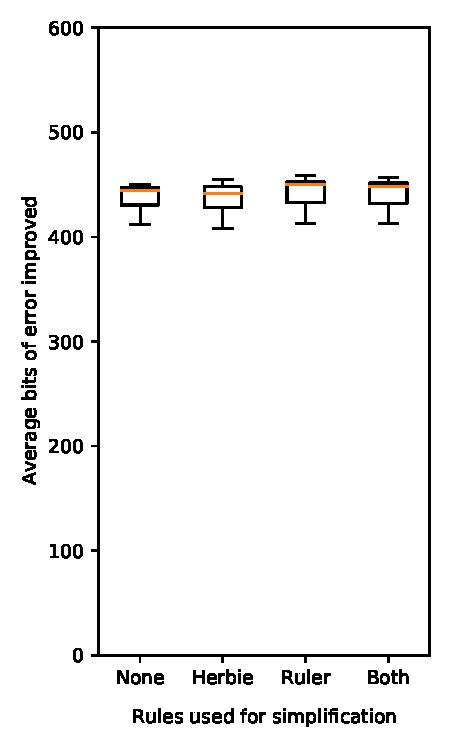
\includegraphics[width=\linewidth]{herbie-ruler/default-error.pdf}
   \caption{
     Improvement in average error,
     Herbie's metric for measuring accuracy
     (higher is better).
    }
\end{subfigure}
\hfill
\begin{subfigure}[t]{0.3\linewidth}
   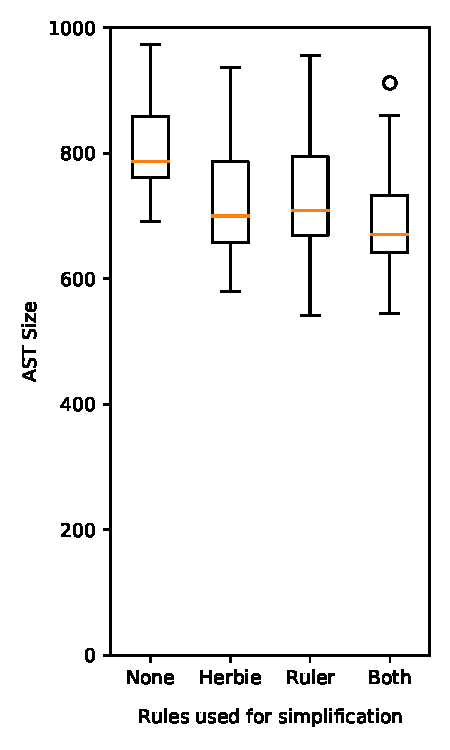
\includegraphics[width=\linewidth]{herbie-ruler/default-ast.pdf}
   \caption{
     Size of the output AST produced by Herbie
     (lower is better).
   }
\end{subfigure}
\hfill
\begin{subfigure}[t]{0.3\linewidth}
  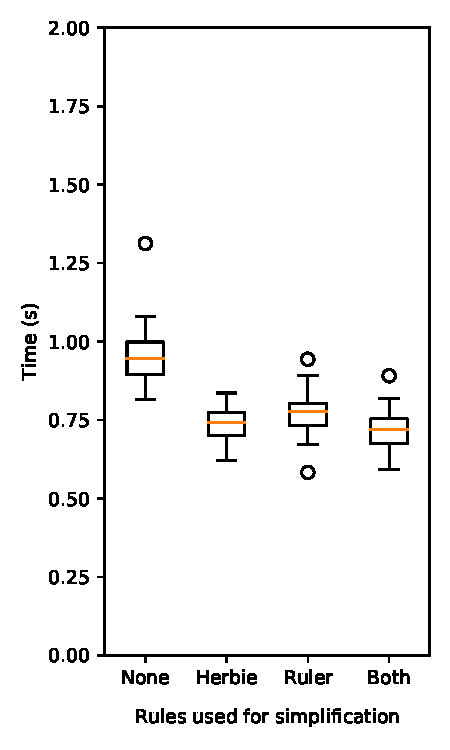
\includegraphics[width=\linewidth]{herbie-ruler/default-time.pdf}
  \caption{
  Herbie's running time (lower is better).
  }
\end{subfigure}
\caption{
 Comparing Herbie results between four configurations.
Each boxplot represents the results from 30 seeds,
 where each data point is obtained by summing the value
 (average error, AST size, time) over all 51 benchmarks.
The columns dictate what rational rules Herbie has access to:
 either none, its default rules, only \ruler's rules, or both.
Herbie's rational rules reduce AST size
 and speed up simplification without reducing accuracy,
 and \ruler's rules perform similarly (with or without Herbie's rules).
}
\label{fig:ruler-herbie}
\end{figure}

\paragraph{Discussion}
The Herbie simplifier uses equality saturation
  to find smaller, equivalent programs.
The simplifier itself does not directly improve accuracy;
  rather, it generates more candidates that are then used in the other
  accuracy improving components of Herbie.
While ideally, Herbie would return a more accurate \textit{and} smaller
 output, Herbie's ultimate goal is to find more accurate expressions,
  even if it sacrifices AST size.
Herbie's original ruleset has been developed
  over the past 6 years by
  numerical methods experts to effectively
  accomplish this goal.
%   and is often updated to include
%   custom rewrites directed towards
%   improving the accuracy specific benchmarks.
Any
  change to these rules
%   automated tool for synthesizing rewrite rules for Herbie,
  must therefore ensure that it does not make
  Herbie's result less accurate.
%   than
%   Herbie's original rewrite rules.
  %in order to be useful and practical for Herbie.

\autoref{fig:ruler-herbie} shows the results of running Herbie
  with rules synthesized by \ruler.
Each box-plot corresponds to one of the four configurations.
The baseline (\lstinline{None}) and
   \lstinline{Herbie}
  in \autoref{fig:ruler-herbie}'s
  accuracy and AST size plots highlight the significance of
  rational rewrites in Herbie ---
  these expert-written rules
  reduce AST size without
  reducing accuracy.
The plots for \lstinline{Ruler}
  show that running Herbie with only \ruler's rational rules
   has almost the same effect on accuracy and AST size
   as Herbie's original, expert written ruleset.
The plot for \lstinline{Both} shows that running Herbie together
  with Ruler's rules further reduces AST size,
  still without affecting accuracy.
The timing plots show that adding \ruler's rules to Herbie
  does not make it slower.
The baseline timing is slower than the rest because
  removing all rational
  simplification rules causes Herbie's other components
  take much longer to find the same results.\\

In summary, \ruler's rational rewrite rules can be easily integrated
  into Herbie, and they perform as
  well as expert-written rules without incurring any additional
  overhead.

% \paragraph{Derivability} Herbie's original rational ruleset consisted of
%   52 rational rules.
% \ruler synthesized 76 uni-directional rational rules (50 bidirectional rules).
% We compared the two rulesets for proving power, by deriving
%   each with the other using the approach described in \autoref{subsubsec:derive}.
% We found that Herbie's ruleset was able to
%   derive 42 out of the 50 \ruler rules.
% It failed to derive the remaining 8.
% \ruler on the other hand, was able to derive all 52 rules from Herbie.
% We highlight two of the 8 \ruler rules that Herbie's ruleset failed to derive
% that concern multiplications interaction with absolute value:
% $(|a \times b| \to |a| \times |b|)$, and
% $(|a \times a| \to a \times a)$.

\paragraph{Fixing a Herbie Bug}

\ruler
 found the following two rules that
 helped the Herbie team address a GitHub issue~\cite{herbie-bug}:
$(|a \times b| \to |a| \times |b|)$, and
$(|a \times a| \to a \times a)$.
In many cases, Herbie may generate large,
 complex outputs without improving accuracy, which makes
 the program unreadable and hard to debug.
This is often due to lack of appropriate rules for
  expression simplification.
The issue raised by a user (\cite{herbie-bug}) was in fact due to the
 missing rule $(|x| \times |x| \to x \times x)$.
The two rules above, can together, accomplish the effect of this
 rule, thereby solving the issue.
We submitted these two rules to the Herbie developers and they
 added them to their ruleset.
